% TEMPLATE for Usenix papers, specifically to meet requirements of
%  USENIX '05
% originally a template for producing IEEE-format articles using LaTeX.
%   written by Matthew Ward, CS Department, Worcester Polytechnic Institute.
% adapted by David Beazley for his excellent SWIG paper in Proceedings,
%   Tcl 96
% turned into a smartass generic template by De Clarke, with thanks to
%   both the above pioneers
% use at your own risk.  Complaints to /dev/null.
% make it two column with no page numbering, default is 10 point

% Munged by Fred Douglis <douglis@research.att.com> 10/97 to separate
% the .sty file from the LaTeX source template, so that people can
% more easily include the .sty file into an existing document.  Also
% changed to more closely follow the style guidelines as represented
% by the Word sample file. 

% Note that since 2010, USENIX does not require endnotes. If you want
% foot of page notes, don't include the endnotes package in the 
% usepackage command, below.

% This version uses the latex2e styles, not the very ancient 2.09 stuff.
\documentclass[letterpaper,twocolumn,10pt]{article}
\usepackage{usenix,epsfig,xspace}
\usepackage[sort,nocompress]{cite}                                     % Sort Citations
\usepackage[protrusion=true,expansion=true,kerning]{microtype}         % Prettier text
\usepackage{soul}                                                      % Provides \hl
%\usepackage[subrefformat=parens,labelformat=simple]{subcaption}        % Replaces both subfig and subfigure
\usepackage{textcomp}                                                  % Provides \textmu for upright mu's

\usepackage[usenames,dvipsnames,svgnames]{xcolor}                      % Allow the use and definition of colors
\usepackage[colorlinks=true,citecolor=violet,urlcolor=blue]{hyperref}  % Creates hyperlinks from ref/cite
\hypersetup{pdfstartview=FitH}                                         % Sets default zoom to 100% width 
\usepackage[capitalise,nameinlink,noabbrev]{cleveref}                  % Do the right thing with fig/table references

\setlength{\textfloatsep}{0.40cm}
\usepackage[compact,nonindentfirst]{titlesec}
\titlespacing{\section}{0pt}{1.5ex}{0.4ex}
\titlespacing{\subsection}{0pt}{1ex}{0.37ex}
\titlespacing{\paragraph}{0pt}{0ex}{1ex}


% Break URLs properly (thanks to Alex Halderman)
\def\UrlBreaks{\do-\do\.\do\@\do\\\do\!\do\_\do\|\do\;\do\>\do\]\do\)\do\,\do\?\do\'\do+\do\=\do\#}
\def\UrlBigBreaks{\do\:\do\/}


\newcommand{\name}{Tock\xspace}

% Some macros that a broadly useful:
\newcommand{\uW}{{\textmu}W\xspace}
\newcommand{\uA}{{\textmu}A\xspace}
\newcommand{\um}{{\textmu}m\xspace}
\newcommand{\us}{{\textmu}s\xspace}
\newcommand{\uF}{{\textmu}F\xspace}
\newcommand{\uJ}{{\textmu}J\xspace}
\newcommand{\iic}{I$^2$C\xspace}
\newcommand{\vdd}{V$_{\textnormal{DD}}$\xspace}

% Command for unnumbered footnote that doesn't increment footnote counter
\makeatletter
\def\blfootnote{\xdef\@thefnmark{}\@footnotetext}
\makeatother

\begin{document}

%don't want date printed
\date{}

%make title bold and 14 pt font (Latex default is non-bold, 16 pt)
\title{\Large \bf Microcontrollers Deserve Protection Too}

\author{
\begin{tabular}{ccc}
  \multicolumn{3}{c}{
    Michael P Andersen$^\dagger$,
    Tom Bauer$^\ddagger$,
    Sergio Benitez$^\ddagger$,
    Bradford Campbell$^\S$,
    David Culler$^\dagger$,
  } \\
  \multicolumn{3}{c}{
    Prabal Dutta$^\S$,
    Philip Levis$^\ddagger$,
    Amit Levy$^\ddagger$,
    and
    Pat Pannuto$^\S$
    %%\vspace{0.3cm}
  } \\
  %
  %\small{$^\dagger$Computer Science \& Engineering} &
  %\small{$^\ddagger$Computer Science \& Engineering} &
  %\small{$^\S$Computer Science \& Engineering} \\
  %
  \small{$^\dagger$University of California, Berkeley} &
  \small{$^\ddagger$Stanford University} &
  \small{$^\S$University of Michigan} \\
  %
  %\small{Berkeley, CA 94720} &
  %\small{Stanford, CA 94305} &
  %\small{Ann Arbor, MI 48109} \\
  %
  \small{\{m.andersen,culler\}@berkeley.edu} &
  \small{\{tbauer01,sbenitez,pal,levya\}@stanford.edu} &
  \small{\{bradjc,prabal,ppannuto\}@umich.edu} \\
\end{tabular}
}

\maketitle

\blfootnote{Authors listed in alphabetical order.}

% Use the following at camera-ready time to suppress page numbers.
% Comment it out when you first submit the paper for review.
%\thispagestyle{empty}

\begin{abstract}


Microcontroller operating systems and frameworks typically assume that a single,
monolithic application will run on an embedded system.
Traditionally, the need to optimize for power and to squeeze applications into
minimal code and memory allocations have constrained microcontroller
applications to be single-function.
The absence of hardware primitives capable of providing protection has
elimintaed security and isolation as considerations.
Newer hardware, however, has changed this paradigm.
The microcontroller is growing up and can now support a secure, trusted kernel
and multiple, isolated, concurrent, and dynamically-loaded applications, all
while operating on the power budgets that originally made this device class
feasible.
While the hardware support is now present, the software ecosystem to
capitalize on these advances is lagging behind.
To remedy this, we propose Tock, a new embedded operating system that builds
on established operating system principles adapted to the embedded system
environment.
Tock exploits memory protection units, advancements in modern systems
programming languages, and the event driven nature of embedded applications to
allow a core kernel, device specific drivers, and untrusted applications to
coexist on a single microcontroller.
This new operating system will allow embedded devices to mature beyond
program-once, deploy-once systems into re-usable, ubiquitous, and reliable
computing platforms.




% This is no
% longer the case with modern hardware. Modern microcontrollers, like the Atmel
% SAM4L (an ARM Cortex-M4), provides over six times more SRAM and over five times
% larger flash than the TI~MSP430 that powered the TelosB motes while maintaining
% similar power draws (90~{\uA}/MHz active and 3~\uA at sleep).
% Simultaneously embedded products are becoming a development platforms and an
% application ecosystems for products like the Pebble watch. Additionally, a set
% of modular embedded devices is emerging. Devices like SimBand, Wzzard and
% ThinkingThings have a core part to which additional modules can be attached to
% extend the functionality. These modules can be developed by the third parties
% and have own microcontroller with runtime environment.
% The operating systems community should leverage advancements in hardware,
% programming languages as well as our experience from the Web, and other
% application rich ecosystems, to build the next generation of embedded operating
% systems.


\end{abstract}

\section{Introduction}

As networking became an integral part of computing through the Internet and
world wide web, system security grew in importance from a niche interest of the
military into a core requirement for operating systems. While far from perfect,
today's general purpose operating systems support firewalls, NATs, encrypted
networking, no-execute bits, randomized memory allocation, signed packages, and a
host of other security features. With the growth in networked embedded
devices, it is time for embedded operating systems to follow suit.

Today, we see the emergence of ``intelligent'' \textit{things} that integrate
computing with physical devices.
% Smart watches such as the Pebble~\cite{pebble}
% provide a clock application and a limited set of applets.
% Smart light bulbs such
% as the Phillips Hue~\cite{hue} support simple functions---turn on, turn blue,
% glow brighter---and personal fitness trackers like Fitbit~\cite{fitbit} and
% UP~\cite{jawboneup} measure our steps, heart rate and sleep
% patterns.
Smart pill bottles such as AdhereTech's~\cite{adheretech} monitor our
medications and remind us of missed doses and wearable personal fitness trackers
like Fitbit~\cite{fitbit} and UP~\cite{jawboneup} measure our steps and sleep
patterns. But the devices are siloed: Fitbit cannot load the ``pill app'' that
vibrates when it is time to take today's medication.
As embedded systems grow from narrow applications into a more general
purpose computing platforms, there will be a need to dynamically load
applications and share the hardware across multiple applications. In fact, this
trend is already underway: the Pebble watch~\cite{pebble}, for example, supports loading
executable code that can use the built-in sensors and display as well as
communicate with apps on a connected mobile phone.

%on and off, brighter and dimmer---,

Traditionally, embedded systems have been single-purpose, single-application
devices. A developer compiles a monolithic application image which incorporates
the OS and gives the application full access to underlying hardware.
The software was co-designed with hardware---i.e. by the same
people---and this paradigm was what the
underlying microcontrollers could support.
Without virtual memory or segmentation features
% Microcontroller families such as the MSP430 and Atmega were simple and
% lacked features of general-purpose processors such as virtual
% memory or segmentation. As a result,
embedded ``operating systems'' have no
security mechanisms and applications must be trusted completely. Even designs
which separate kernel and application code~\cite{han05sos,contiki,freertos}
require trusted applications.

However, a new generation of microcontrollers has emerged recently.
These processors, based on the ARM Cortex-M architecture, sit in a middle ground
between full-fledged CPUs and older microcontrollers. Like some mid-1980s processors,
they have a 32-bit address space, memory protection, and run at tens of MHz.
Like microcontrollers, they have tens to a few hundred KB of RAM, provide many
peripherals and bus interconnects (SPI, I2C, one-wire, UART/USART, etc.) and
have sub-\uA sleep currents, allowing them to operate on a battery for
months or years. The Atmel SAM4L~\cite{sam4l}, for example, is a
microcontroller with a Cortex-M4 processor (40~MHz, 64~KB RAM, 512~KB flash), a
plethora of peripherals (4 USARTs, 2 SPIs, 6 timers, native AES and a random number
generator) and has a sleep current as low as $0.9$~\uA.

Most importantly to an operating system, this new generation of microcontrollers includes
memory protection.
This can protect kernel memory, memory-mapped I/O, and
application memory from misbehaving applications. However,
isolation and safety is only as good as the kernel itself. As numerous recent
results show, OS kernels contain scores of memory access bugs that applications
can exploit to crash a system or gain unauthorized
access~\cite{kint:osdi2012,linuxvulns:apsys11}. By writing the OS kernel in a
type-safe, memory-safe language with strong semantics, we can eliminate whole
classes of vulnerabilities. The relative simplicity of Cortex-M processors and
embedded operating system APIs means that writing such a kernel is a
manageable task.  This makes an embedded OS especially well suited for
research in secure operating systems design.
% still open to easy extension and evolution.

It is time for embedded operating systems to evolve! In this paper, we argue
that an embedded operating system should be more than a hardware API.
It should enable and encourage
multiple concurrent, isolated applications, provide  hardware abstractions
as well as low-level hardware access, and offer critical services to Internet
of Things applications. We discuss three protection
mechanisms---language level isolation, software mediated hardware protection, and
multiple isolated processors---that operating systems should utilize to achieve
these goals.

%(alevy): I don't think we need this in the intro.
%As a concrete example of what such an operating
%system might look like, we present \name, a new operating system that combines
%hardware-based memory protection and language-based safety to provide a secure,
%robust platform for embedded applications.

% Sergio's note: This isn't particularly difficult since we've already discussed
% that the kernel and applications will be isolated by hardware. The language
% the applications are written in is irrelevant when this is the case.
%
% The principal challenge that arises is safely and correctly
% integrating untrusted application code in C with a type-safe kernel,
% particularly in how data passes between them and how the OS manages its memory
% layout.

\section{Operating System Considerations}
\label{os-considerations}
%\subsection{Evolved Embedded Applications}

In a first evolutionary cycle of the embedded devices applications were written
as a essential part of a runtime environment on the device. During secondary
cycle operating systems like TinyOS, Contiki, FreeRTOS emerged separating
application and OS spaces. The development became easier  and applications
got complex but the resulting code was still compiled to a monolithic image and
uploaded to the device.

Now the third evolutionary cycle is emerging: multiple and independently
developed application has to co-exist on the same device (like in Pebble watch);
and embedded devices are becoming modular. The later is evident with
multi-billion companies like Samsung, Telefonica and GE innovating with SimBand, Wzzard, ThinkingThings, Spotter UNIQ.
%~\endnote{http://www.samsung.com/us/globalinnovation/innovation_areas/}, Wzzard
%~\endnote{http://bb-smartsensing.com/wzzard-sensing-platform/}, ThinkingThings
%~\endnote{http://www.thinkingthings.telefonica.com/}, Spotter UNIQ
%~\endnote{https://www.quirky.com/shop/982-spotter-uniq-customizable-multipurpose-sensor}
The aim is to create a core hardware platform where adding sensory
peripherals is done by consumer in a Lego-like fashion while developer compiles
application with provided SDK.

These trends completely change the way applications for the embedded devices
have been developed last five decades. Developer have very little control on the
application execution model, its coexistence with other application and what
peripherals are connected to the embedded device. Instead application developer
expect that underlying operating system will perform fair resource allocation,
protect the application from malicious or malfunctioning applications and
peripherals. 

Given the paradigm shift in embedded devices we design new operating system
\name that supports a combinations of goals:


\begin{itemize}
  \item Event-driven execution model
  \item Loadable applications, services and drivers
  \item Robust, Reliable and Safe %isolation
  \item Energy Efficient 
\end{itemize}



\subsection{Application execution model}
\begin{figure}
 \centering
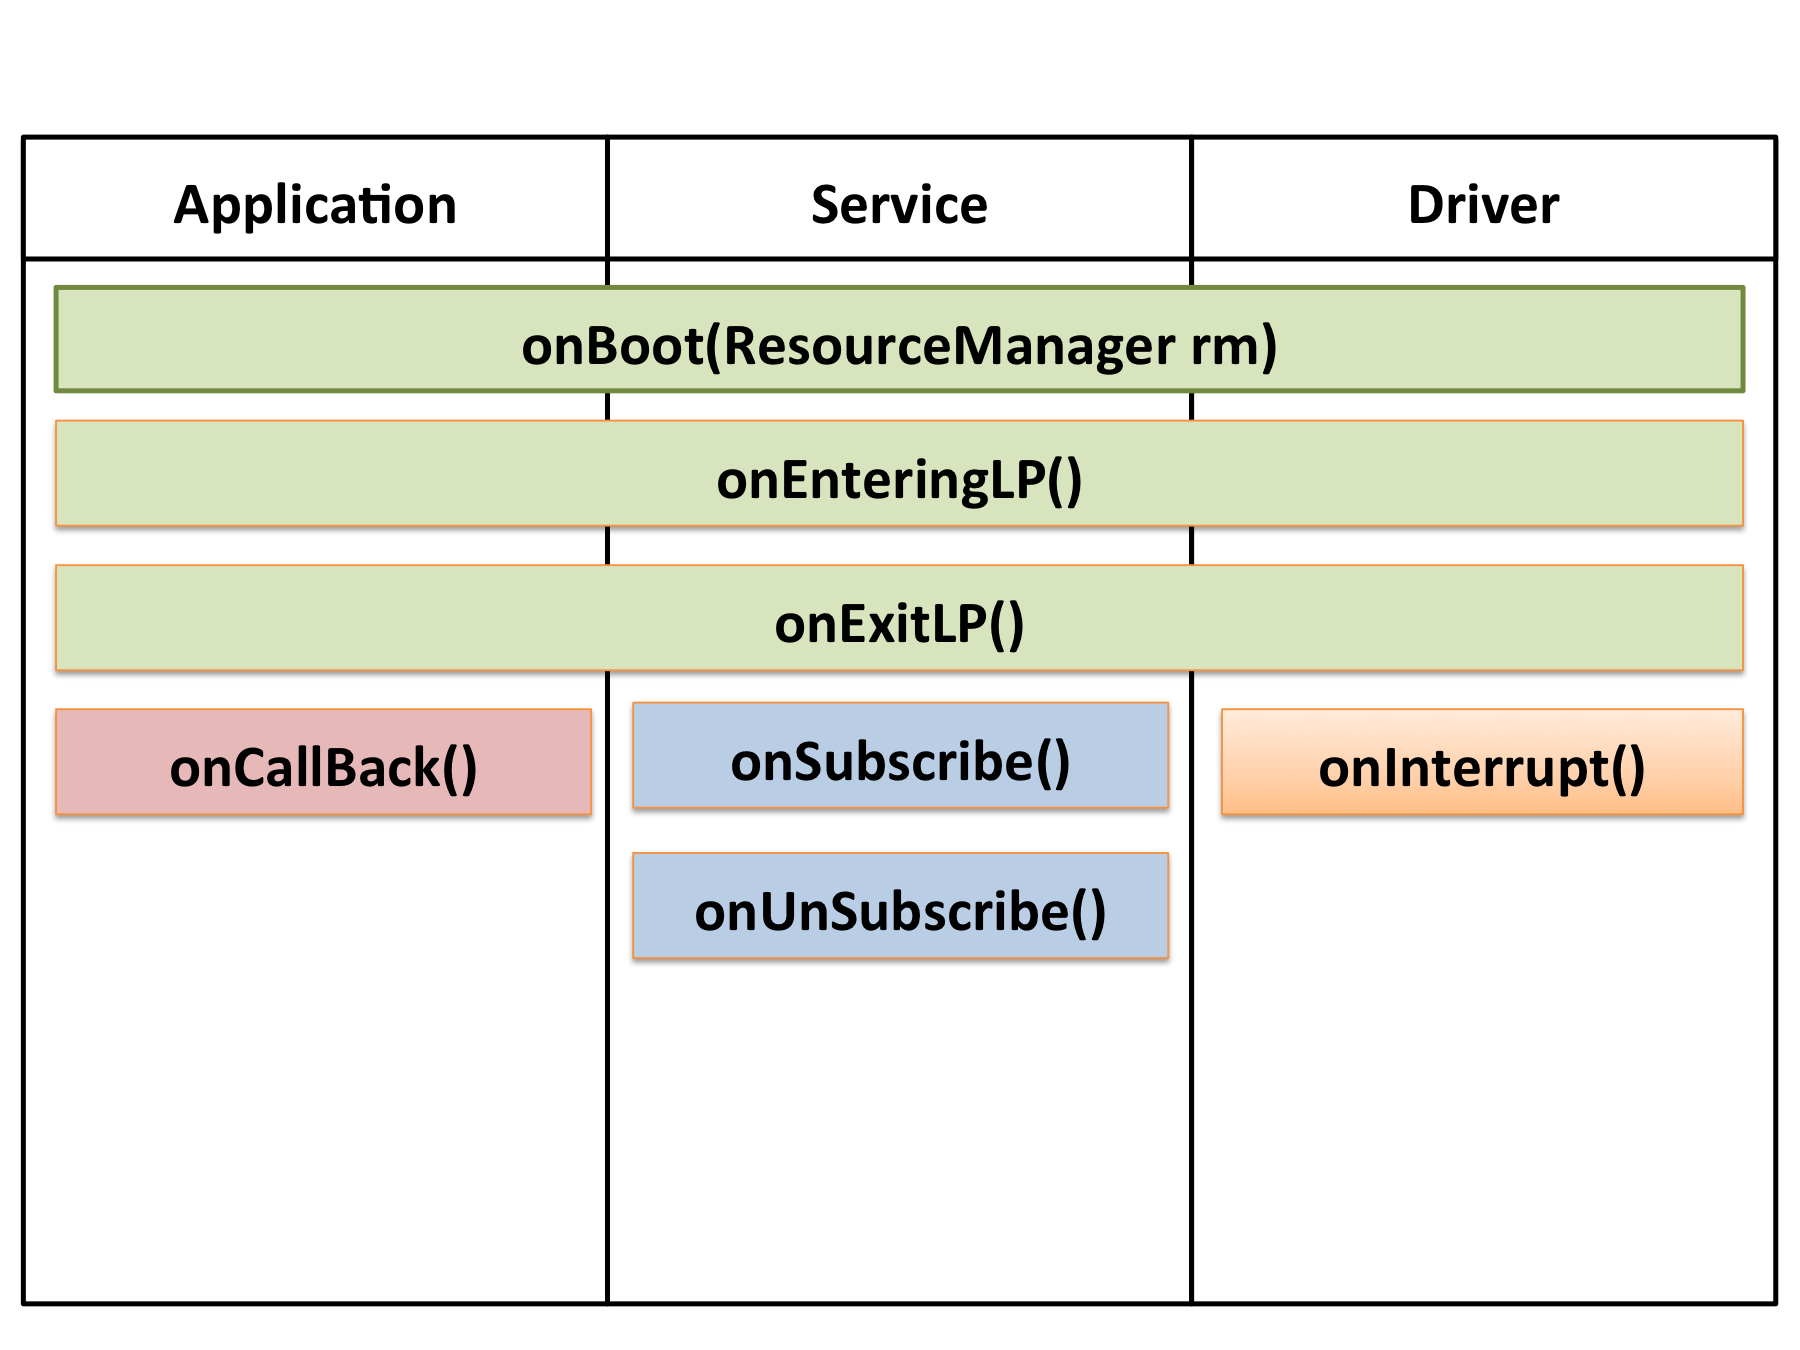
\includegraphics[width=1\columnwidth]{img/appcycle.png}
\caption{Runnable life cycle.}
 \label{fig:appcycle}
\end{figure}


\subsection{Loadable applications, services and drivers}

\name provides a system-call interface. This
allows developers to write applications in any language that can support the
ABI. For example, the \name kernel is written in Rust~\cite{rust}, applications
can trivially written in C, and we are working on a port of Lua~\cite{lua}.

\subsection{Robust, Reliable and Safe}
%tobe rewriten
 \name follows previous operating systems in separating
drivers for core peripherals (SPI, USART, GPIO, etc) and device drivers (radio,
flash, etc) into separate layers. \name differs from previous operating systems
in enforcing safety policies on device drivers through the Rust type system.
\name prevents drivers from subverting Rust's memory safety by restricting
device drivers to a safe subset of the Rust language.~\endnote{Rust allows code
to circumvent the type system using the \tt{unsafe} keyword. \name uses a
compiler flag that disallows this keyword when compiling device drivers.} \name
also ensures, at compile time, that at most one driver has access to a specific
hardware resource---multiplexing must be done explicitly in the core peripheral
driver or through an intermediate interface. Finally, \name ensures device
drivers cannot corrupt kernel memory through careful choice of interfaces. \name
ensures that \name does not protect the kernel from denial of service attacks by
drivers.

{\bf Reliability}. Unlike most desktop and server applications, embedded
applications must continue to run without end-user intervention. There is no
console to indicate to the user that an application has crashed. Even if a crash
could be communicated to the user, there is little action she could take. While
a Blue-Screen-Of-Death is annoying on a desktop or server, it is unacceptable in
embedded systems. Unlike other embedded operating systems, in \name,
applications cannot corrupt the kernel or other applications. Moreover, certain
parts of the kernel (e.g. contributed device drivers) are isolated using
a strong language type system.

\subsection{Energy Efficient}


\subsection{Scheduling}



\section{Protection \emph{is} a New Primitive}

% pp 33--34, ch 1, sec 4:
In Tanenbaum's \emph{Modern Operating Systems} he asserts, ``The main property
which distinguishes embedded systems from handhelds is the certainty that no
untrusted software will ever run on it''~\cite{tanenbaum}. In this paper we
argue that this is no longer the case. As a class of device, embedded systems
are evolving beyond the single-application case, and as a consequence, they
require their operating system to provide process isolation, enforced resource
arbitration, and protection.
%
Three converging trends, modern language design, new microcontroller hardware
primitives, and contemporary multi-MCU system design afford new opportunites
to provide protection as a primitive that was previously unavailable to
embedded systems.



\subsection{Language Level Protection}

\name is written in Rust: a type-safe, thread-safe, compiled, low-level systems
language. Using a language with strong safety protections has enabled \name to
formalize the separation between core kernel code and contributed device
drivers, which are traditionally where most bugs are found but are included in
the kernel for performance and practical reasons. While recent server operating
systems utilize hardware I/O virtualization~\cite{arrakis:osdi2014, ix:osdi2014}
to run device drivers outside the kernel, such hardware mechanisms are unlikely
to be available in microcontrollers in the foreseable future.

\subsection{Memory Protection}

Modern ARM Cortex-M processors provide a hardware protection mechanism called
Memory Protection Unit (MPU).  An MPU allows the kernel to set access
permissions on a fixed number of memory regions which are enforced on
application code. Like Memory Management Units (MMUs) found in application
processors, MPUs trap illegal memory accesses (e.g. writing to read-only memory)
to the kernel, however unlike the MMUs, they do not provide virtual addressing,
so do not enable mechanisms like swap memory, shared libraries, etc. MPUs are
typically much more fine-grained than virtual memory. For example, in the ARM
Cortex-M series of microcontrollers, the MPU can address regions as small as 32
bytes, whereas virtual memory typically divides memory into pages of at least
4KB.

\name uses the MPU to protect kernel and driver memory from untrusted
application code as well as different applications from one another.
Applications are given dedicated region of memory for stack, heap and appliction
specific kernel buffers. When execution is yielded to an application, the MPU
restricts access to memory outside of this region. Moreover, application
specific kenel buffers (e.g. interrupt callback queues) are allocated in the
application's memory region, but protected from application tampering. This is
possible due to the fine granularity of the MPU and allows \name to eliminate
dynamic allocation in the kernel but allow more runtime flexibility in
applications.

In contrast to traditional embedded operating systems, \name uses a system call
ABI rather than library calls to provide an interface between applications and
the kernel.

\subsection{Multiple Processors}

Modern embedded platforms often involve multiple microprocessors in practice.
For example, both the CC2540 and the NRF51822 Bluetooth modules are, in fact,
full blown microprocessors, but many products include them in addition to
another microprocessor~\endnote{Well, at least Coin does that}. Tock leverage
multiprocessor environments to enforce another layer of isolation between
applications and the kernel, by running different application components on
different cores depending on their needs to access specific hardware, as well as
power and performance constraints.


\section{\name: a Secure Embedded OS}
\label{sec:os}

\name is a new embedded operating system specifically designed for platforms
running multiple applications concurrently on platforms with multiple
microcontrollers. \name's design centers around protection---from potentially
malicious applications and from buggy device drivers. \name uses three
protection mechanisms to protect three different components in the operating
system. First, the kernel and device drivers are written in Rust~\cite{rust}, a
new systems language that provides compile-time memory safety, type safety and
strict aliasing. \name uses Rust to protect the core of the kernel (e.g. the
scheduler and hardware abstraction layer) from platform specific device drivers
as well as isolate device drivers from each other. Second, \name uses new Memory
Protection Units (MPUs) to isolate third-party applications from each other and
the kernel. Finally, where available, \name uses multiple microcontrollers to
protect applications with timing concerns against starvation or leaking
information through side-channels. The remainder of this section gives an
overview of the \name architecture, and aims to provide some intuition for the
importance and usage of an MPU.

\subsection{Architecture}
\label{sec:os-arch}

\begin{figure}
 \centering
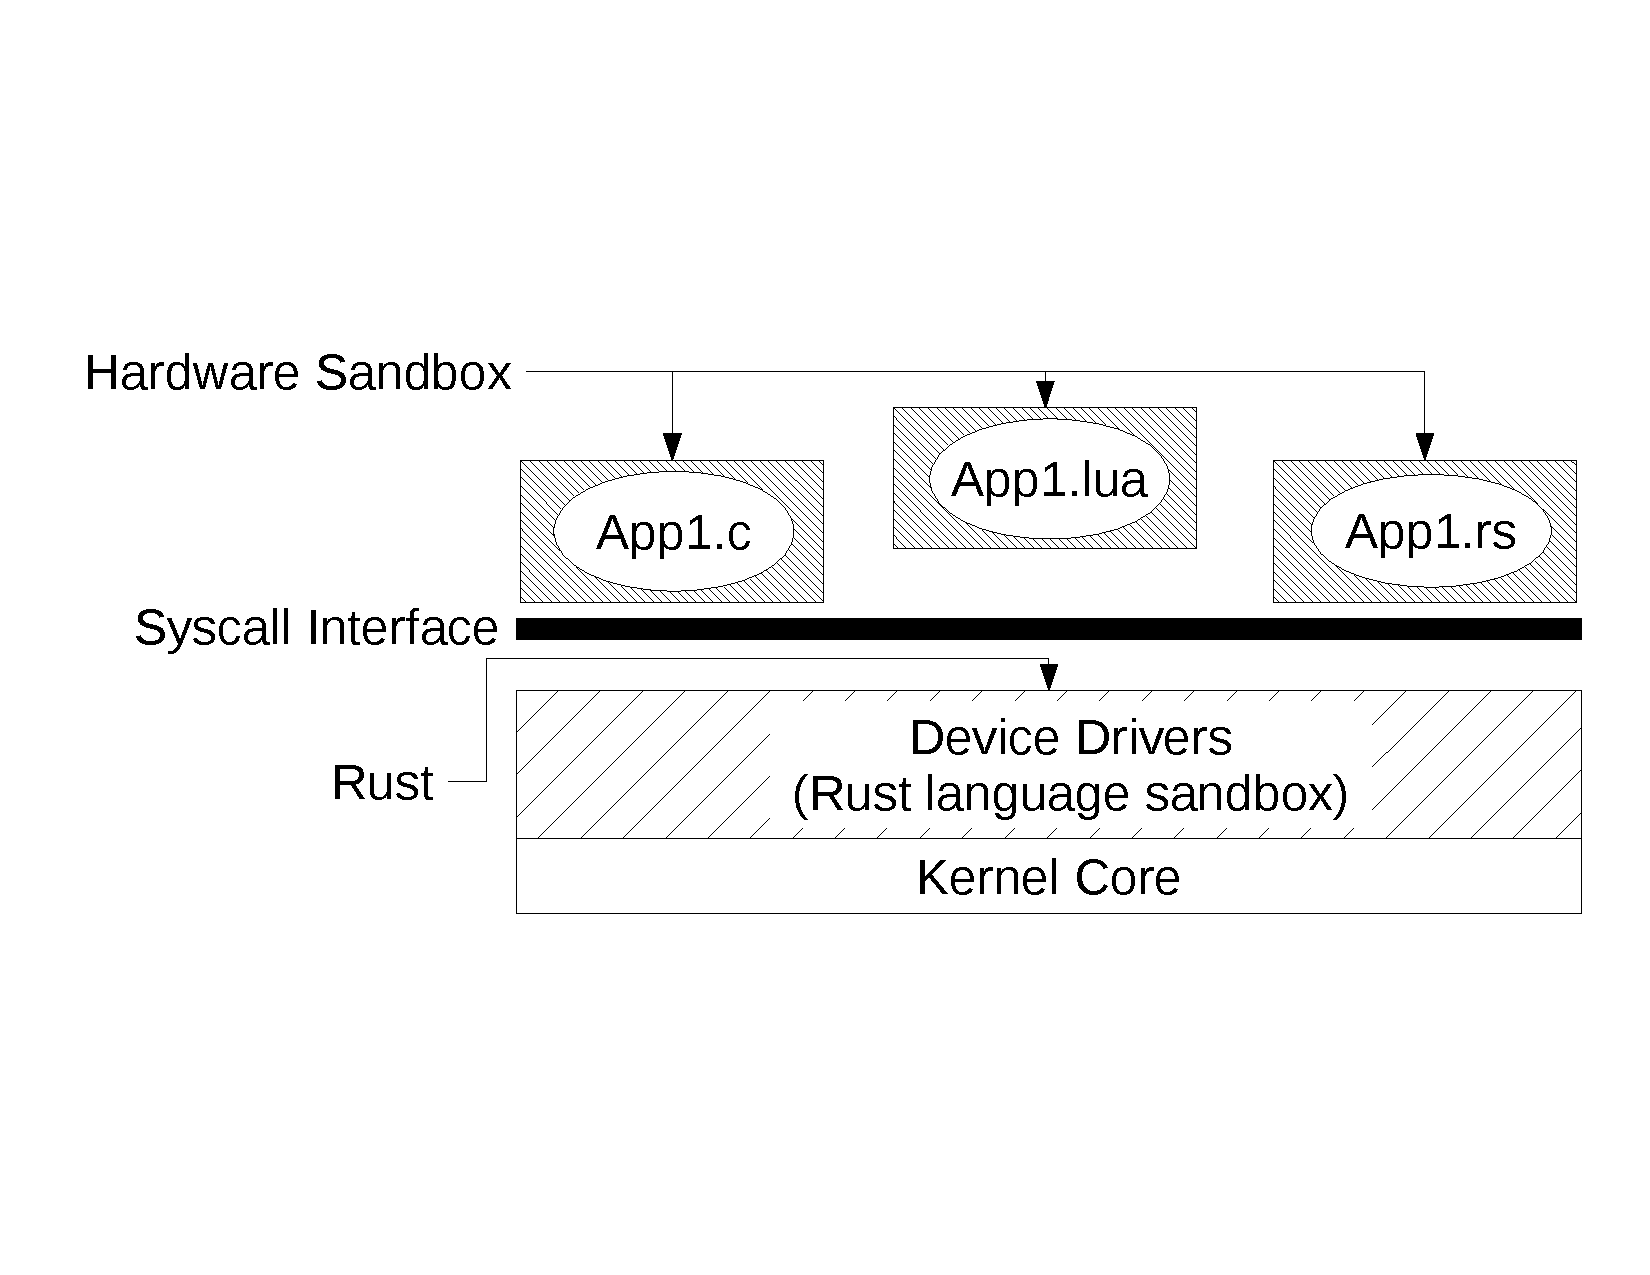
\includegraphics[width=1\columnwidth]{img/architecture}
\caption{\name is written in Rust, a type-safe, memory-safe systems language.
The \name kernel's core has full access to the underlying hardware. Device
drivers run with no hardware protection, but within a language sandbox that
constrains their access to hardware. Applications are sandboxed using the MPU, a
hardware memory protection mechanism, and can be written in any language (e.g.
C, Rust, or even a scripting language like Lua).}
\label{fig:architecture}
\end{figure}

% Definitions:
%  Tock core -- the kernel code shipped and provided with base Tock
%  Tock kernel -- the final compiled kernel, including core and drivers

The \name core has complete system access, including arbitrary memory
access and interrupt control. Device drivers are compiled into the kernel and
run with the same \emph{hardware} privileges but inside a
\emph{language-level} sandbox. This sandbox statically enforces that device
drivers only use core-provided hardware interfaces, limits dynamic memory
allocation to load time, and prevents uncoordinated access of underlying
hardware resources.

Applications are separated from the kernel by a syscall ABI and need not be
written in Rust. Applications have an execution stack, an application memory
heap, and a kernel memory heap. Kernel (and driver) dynamic allocations take
place in the application memory space, thus charging applications for buffers
the kernel creates on their behalf and ensuring that an out-of-memory
condition terminates the application and does not cause a kernel error. The
application-level kernel memory heap is protected from application access by the
MPU.
%
The ABI provides access to system hardware resources. For embedded applications,
however, direct access to a hardware peripheral is often required.
Applications can request direct ownership, in which case the kernel uses the
MPU to grant the application access to the memory mapped I/O region of
specific peripherals.

%% Brad: not sure what this paragraph contributes to the paper, particularly
%% in this section. I think the contents of this should be discussed in the sections above, if
%% at all.
% Scheduling in \name is an open question, particularly if it aims to capitalize
% on multi-MCU systems. Some assignments are clearer, a communication task
% should likely run on the same core as the radio controller. Applications
% that require hard real-time could run on a dedicated core with a real-time
% scheduler, but what if another core is not available? Technology such as
% TrustZone~\cite{trustzone}, a secure processing mode on the same physical
% core, provides protection for sensitive data, but not from side-channel
% attacks such as timing.


% TrustZone is interesting, but currently only available on Cortex-A's, not
% clear if there's any intention of bringing to M's. Maybe this though belongs
% more in the HW section earlier?


% \subsection{The Cortex-M MPU}
%
% The Cortex-M MPU allows the kernel to defined eight memory regions. Each memory
% region may be sized between 32 bytes and 4GB, in 32 byte increments and has
% protection bits for read, write and execute. Regions may overlap, in which case
% the memory region with the highest number ``wins''. In addition, regions of at
% least 256 bytes can be divided into eight equal sized subregions, which can
% either be turned on---in which case they inheret the parent region's protection
% bits---or turned off---in which case the parent's protection bits do not apply.
% As a result, the operating system can control access to up to 64 concurrently
% active regions. Finally, memory regions and protection bits can be changed
% during exection, for example while context switching between applications.


\subsection{\name Memory Design in Detail}


\begin{figure}
 \centering
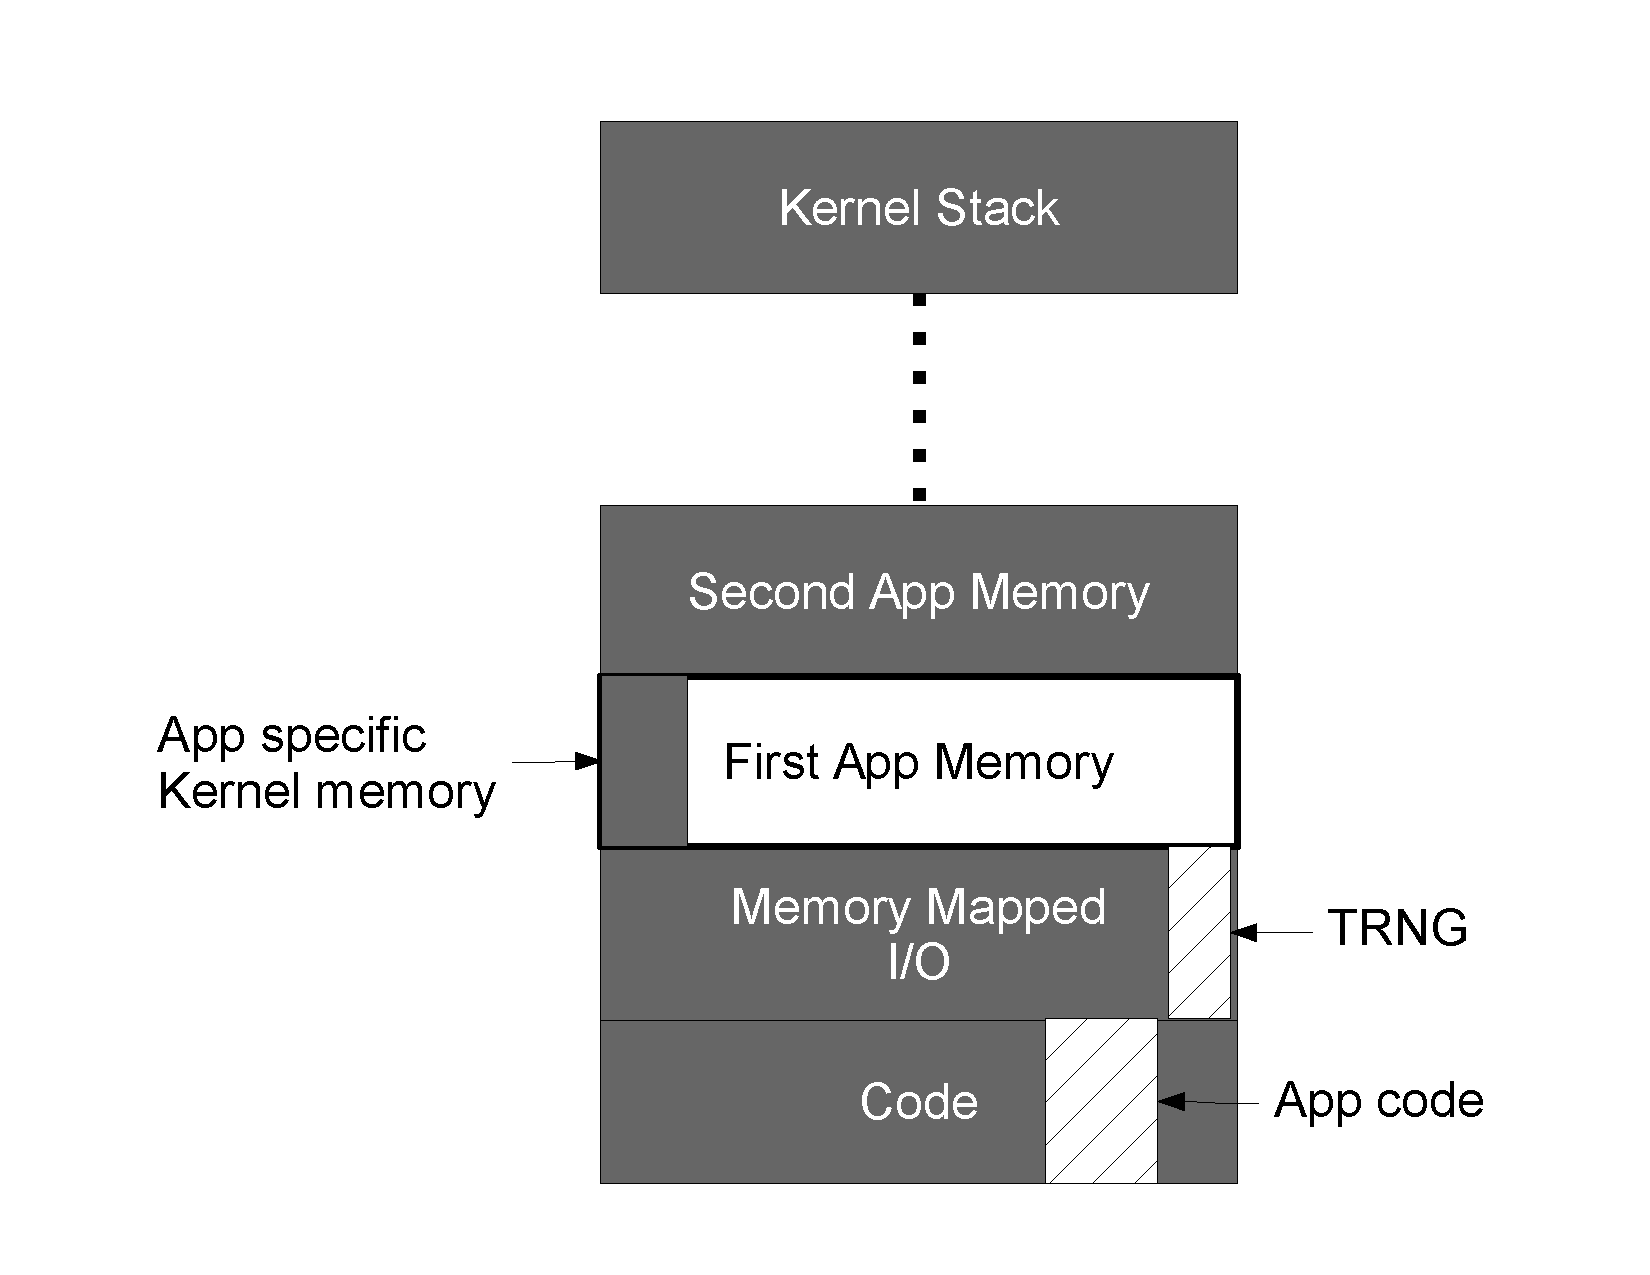
\includegraphics[width=1\columnwidth]{img/memory-layout}
\caption{Memory layout and access permissions while executing an application.
\name lays out memory into four types of regions: code, memory mapped I/O,
application memory and the kernel stack. Greyed regions are marked unreadable
and unwritable, while hatched regions are read-only. The application memory
contains a subregion used by the kernel for application-specific kernel data
structures and is thus inaccessible to the application. Conversely, some
hardware registers are exposed directly to applications by marking them
read-only.}
 \label{fig:memory-layout}
\end{figure}

Tock has four types of memory regions, code regions, memory-mapped I/O regions,
kernel stack and static data regions and application regions.
\Cref{fig:memory-layout} shows these regions and their access rules from
an application.

{\bf Code.}
The code region contains kernel and application code. While an application is
executing code, it only has read and instruction fetch access to its own code
segment. An application cannot write to its own code section because typically
the code is backed by internal flash, which has limited write cycles.

% n.b. Why endnotes? I looked around the HotOS CFP, and couldn't find anything
% that requires them over footnotes. They're much more annoying to read IMHO.
{\bf Memory-Mapped I/O.}
Hardware registers are typically located in a single, continuous region of the
memory space.~\endnote{The location of hardware memory registers and flash is
determined by the chip manufacturer, however, chips chips typically place
flash at the bottom of memory, followed by RAM, and peripheral memory
registers towards the top of memory.} \name may provide read-only or read-write
access over small ranges of memory registers to applications, bypassing the
kernel for direct hardware access. For example, our development platform uses
the Atmel SAM4L Cortex-M4~\cite{sam4l} which provides a true random number
generator (TRNG) peripheral. \name exposes random numbers directly to
applications by allowing read-only access to wthe TRNG registers.

{\bf Kernel Stack and Static Data.}
This section includes all kernel and device driver memory, including local
variables. The MPU restricts any application-level access to this memory section.
% buffers and any local
% variables such that applications may not access the kernel stack in any way.
% The kernel does not allocate memory dynamically except on the stack and inside
% application memory regions.
%As a result, the kernel stack is the only region dedicated to kernel memory.

{\bf Application Memory.}
Currently, \name allocates a continuous, fixed size region for each
application.
%(our development platform has 64KB of RAM and we currently use 2KB
%memory regions for applications, but this will likely vary based on the
%requirements of each target platform).
Application memory and the kernel stack grow towards each other to balance
application count with kernel stack size. If the kernel stack
grows too large, \name terminates the application with the
largest memory region. We intend to explore an alternate strategy of
allocating application memory from a shared heap using the
high granularity of the MPU.
This would trade-off
% We have not yet explored the tradeoffs between
% these two strategies, but at a high level fixed sized application memory
% regions make it
a simpler processes for reclaiming stack space
for better support of heterogeneously sized applications.


An application's memory region is not entirely its own. Most of its memory is
used for its stack, static variables, and heap. However,
the kernel may also ``borrow'' memory from the top of an application's memory
region for application-specific kernel data structures. This region, which may
change in size,
%is \emph{inside} the application's memory space, but
is marked
as read and write protected when the application is running. Therefore, the
kernel and device drivers can allocate memory dynamically in response to an
application without
potentially causing an out-of-memory kernel error and while still
% sacrificing the reliability of never dynamically
% allocating in the kernel itself and while
maintaining the integrity and
confidentiality of shared kernel data structures. As an example, when an
application registers a callback for a timer, the timer device driver
allocates a new link node for the callback in the application's memory.
% adds the
% request to its list of pending timers by allocating the new list node in the
% application's memory.
Since the link includes forward and backward list
pointers, it is imperative that, despite being in the application's memory,
this link's integrity be maintained. Moreover, the values of the links might
leak information about other applications.


\section{Related Work}

Embedded systems have historically had highly fragmented application domains,
each with a vertically integrated set of software and technology that
applications can highly customize as needed. However, until now, a common
assumption in almost all embedded systems is that a single group of developers
is responsible for all of the code running on a device. They might borrow
or use libraries or operating systems from elsewhere, but that code is 
completely under their control to modify and inspect as needed. Making
this assumption means that embedded operating systems typically have
minimal or no system security to protect themselves from malicious code
or applications.

One extreme example of this approach is TinyOS, which makes no
distinction between application and operating system code. Application
code specifies which abstractions and services it needs from the
operating system, and the compilation toolchain uses this information
to build an application-specific version of the OS that is compiled
and directly linked with application code~\cite{tinyos}. Later
versions of TinyOS included a threading library with which one could
dynamically load and link applications~\cite{tosthreads}. These
threads, however, operate under the assumption that the application
developer and the system maintainer are the same person: there are no
security checks and since there is no memory protection applications
have unlimited access to the entire system.

The Contiki operating system is another microcontroller-based
operating system. It has led TCP/IP integration with embedded systems
through libraries such as the $\mu$IP stack and a fully
certified IPv6 stack contributed by Cisco in 2008~\cite{contiki}. 
Security in Contiki is limited to
link-layer encryption and integrity and the OS does not support
dynamically loaded applications. 
%% again this is not true contiki supports dynically loaded code.

FreeRTOS is an open-source commercial operating system intended to 
support a wide range of applications on many different processors. It
is used in applications from the Nest Protect to smart meters to
thermal monitoring systems. FreeRTOS supports for network security
through TLS~\cite{tls} and DTLS~\cite{dtls}, but operates under the
assumption that all code is trusted. For example, any task in the system
can spawn a task that runs in privileged mode and arbitrarily modify
% http://www.freertos.org/a00125.html
% http://sourceforge.net/p/freertos/discussion/382005/thread/7b135e95
the system~\cite{rtos-tasks,rtos-sec}.


%\section{Hardware Considerations}

\begin{enumerate}
\item \bf{Memory Protection Units (MPUs)}

\item \bf{Many More Peripherals}

\item \bf{Multi-core Platforms}
\end{enumerate}

%\section{Challenges}

\subsection{Using a Safe Programming Language}

\begin{enumerate}
  \item Accessing globals is fundamentally part of operating systems development
    (e.g. hardware memory registers), but access to global variables is not
    thread-safe and therefore considered ``unsafe'' in languages like Rust.
    While there is prior art wrapping an unsafe core with an safe interface,
    it's not clear where to draw the line -- which code should be trusted with
    access to unsafe features?

  \item Certain common constructs in high-level programming languages like
    closures often rely on dynamic allocation outside the stack. Embedded
    operating systems usually avoid allocating memory dynamically since memory
    is usually limited in embedded environments and the kernel cannot rely on
    user intervention to recover from fatal runtime errors---instead embedded
    operating systems prefer to rely on compile-time guarantees that memory
    requirements are met.

  \item Other concerns
\end{enumerate}

\subsection{Doing Without Virtual Memory}

\begin{enumerate}
  \item Swapping due to memory use
  \item Allocating application memory. Specifically, virtual memory affords the
    operating system the ability to allocate pages dynamically to an application
    as it requires them (for example, dynamic stack growth in high-level
    languages). This is harder without virtual memory since memory that appears
    continuous to applications {\emph must} be continuous in physical memory.
    Moreover, relocating memory would require changing pointers in application
    code and data structures.
\end{enumerate}

\subsection{Heterogenous Platforms}

Platforms with multiple microprocessors are not like multi-core desktop
operating systems. They typically do not share caches or even main memory.
Often microcontrollers, while from a similar family (like the cortex-m) have
different manufaturer specific features and configurations or are different
architecture versions. As a result, we cannot trivially move work from one
processor to another since that would require relocating memory pointers and
code may simply not be portable.

%\section{Abstractions}

The basic unit of program composition in Tock is a protection domain. A
protection domain describes a set of access rights to physical memory. 

There are be one or more event queues. Every event is associated with
a protection domain and executes within it when it begins. An event
may cross into another protection domain through a function call
(language protection) or a call gate (software protection), or
may invoke it asynchronously through a message (software protection,
hardware protection).

For example, the operating system kernel runs in one protection domain,
which has access to private kernel memory and a region of memory used to
pass messages to the kernel. The kernel memory is not accessible by other
domains, but the message memory is. The kernel reserves the IO pins and buses
that control its peripherals (e.g., the radio, the bus to another core). 

An application runs in another protection domain. It has access to its own
memory, the kernel message memory, and the subset of IO pins and buses
which the kernel does not manage/control.

The operating system can be broken into multiple protection domains. For
example, on Firestorm, any code running on the squall must be in a different
protection domain than code running on the storm core. Like a microkernel
architecture, the OS can invoke core services in separate protection domains.
The decision of whether to place drivers/etc. in the main OS protection domain
or in other domains is driven by a combination of security concerns and 
hardware capabilities.

When a developer writes an application, it consists of potentially multiple
protection domains, some in the form of libraries, some in the form of
application code, some in the form of drivers. The development environment
decides how to divide this code across the cores based on harwdware capabilites
and software operations. E.g., a filter on Bluetooth messages will likely be 
placed on the squall, while the IPv6 stack will likely be placed on the storm.


{\footnotesize \bibliographystyle{acm}
\bibliography{bibliography}}

\end{document}


